\subsection{Comparison with generator predictions}
\label{sec:fived16-gen}
Table~\ref{tab:fived16-gen} compares the result with five generator predictions. Each gives the $\chi^2$ against the reported covariance plus $V_g$, $C_{\mathrm{total}}+C_{\mathrm{resp}}+C_{\mathrm{PL,5D}}+V_g$, where $V_g$ is the prediction's finite-sample (diagonal) covariance, and the shape-only $\chi^{2}$, using the finite penalty $100\,f f^{T}$ (\S\ref{sec:fived16-cov}), which approximates a free normalization, and both again without $C_{\mathrm{PL,5D}}$ (\S\ref{sec:fived16-pl}). No diagonal-only $\chi^2$ is formed. GiBUU's sample has no events above $E_\nu=\fvval{cmodel-gibuu-enu}$~GeV, so it is compared on the 8 cells below $\pPar=\fvval{h2-mid-pz}$~GeV/$c$ only, and no value is formed on the other 8. In the GENIE CV and NuWro samples, at least \fvval{gagg-genie_cv-hi}\% and \fvval{gagg-nuwro-hi}\%, respectively, of the cross section above $\pPar=\fvval{h2-mid-pz}$~GeV/$c$ comes from $E_\nu>\fvval{gagg-ecut}$~GeV. Between $\pPar=\fvval{gagg-pz-lo}$ and \fvval{h2-mid-pz}~GeV/$c$, they are \fvval{gagg-genie_cv-lo}\% and \fvval{gagg-nuwro-lo}\%. These GENIE CV and NuWro fractions, not GiBUU values, are what a sample stopping at $E_\nu=\fvval{gagg-ecut}$~GeV would miss.

All five predictions are in the analysis definitions of $W$ and of the muon angle, and NuWro and GiBUU, generated on carbon, are compared on carbon, as in the methods paper. Corrected to CH by adding each generator's own free-proton prediction with weight \fvval{g-ch-hweight} per nucleon, they give a secondary comparison only (\S\ref{sec:fived16-gen-target}), because the free-proton samples used for the correction have the unresolved validation problems of \S\ref{sec:joint5d-ch}. The per-cell pulls, the correlation sensitivities and the eigenmode breakdown (Tables~\ref{tab:fived16-pulls}--\ref{tab:fived16-diag}) were computed with that CH correction, as their labels show. MINERvA Tune~v1 is the simulation's prior, not an independent prediction. Because $C_{\mathrm{model}}$ holds the GENIE + MEC, NuWro and GiBUU shifts, those comparisons each use a covariance built in part from the compared generator, and the GENIE CV comparison does so through the reference of the ratios.

\begin{table}[htbp]
\centering\footnotesize
\caption[Sixteen-cell comparison with generator predictions]{The comparison with the five generator predictions is descriptive; each $\chi^2$ is in the table. $\chi^2$ against the reported covariance plus $V_g$, $C_{\mathrm{total}}+C_{\mathrm{resp}}+C_{\mathrm{PL,5D}}+V_g$, where $V_g$ is the prediction's finite-sample (diagonal) covariance, with the shape-only $\chi^2$ beside it, and the same two without the run-period block, against $C_{\mathrm{total}}+C_{\mathrm{resp}}+V_g$. All five predictions are in the analysis definitions, with NuWro and GiBUU on carbon, as in the methods paper. Their CH-corrected values are in Table~\ref{tab:fived16-gen-target}, with the caveat of \S\ref{sec:joint5d-ch}. The ndf of each block is given in its heading.}
\label{tab:fived16-gen}
\begin{tabular}{@{}lcccc@{}}
\toprule
 & \multicolumn{2}{c}{reported covariance} & \multicolumn{2}{c}{without $C_{\mathrm{PL,5D}}$} \\ \cmidrule(lr){2-3}\cmidrule(l){4-5}
prediction & $\chi^2$ & shape-only $\chi^2$ & $\chi^2$ & shape-only $\chi^2$ \\
\midrule
\multicolumn{5}{@{}l}{All 16 cells: ndf \fvval{g-gcv-total-ndf}, shape-only \fvval{g-gcv-shape_only-ndf}} \\
\fvval{label-gcv} & \fvval{g-gcv-total-chi2} & \fvval{g-gcv-shape_only-chi2} & \fvval{g-gcv-total-chi2-nopl} & \fvval{g-gcv-shape_only-chi2-nopl} \\
\fvval{label-gmec} & \fvval{g-gmec-total-chi2} & \fvval{g-gmec-shape_only-chi2} & \fvval{g-gmec-total-chi2-nopl} & \fvval{g-gmec-shape_only-chi2-nopl} \\
NuWro~21.09 (carbon) & \fvval{g-nuwro-carbon-total-chi2} & \fvval{g-nuwro-carbon-shape_only-chi2} & \fvval{g-nuwro-carbon-total-chi2-nopl} & \fvval{g-nuwro-carbon-shape_only-chi2-nopl} \\
\fvval{label-tune} & \fvval{g-tune-total-chi2} & \fvval{g-tune-shape_only-chi2} & \fvval{g-tune-total-chi2-nopl} & \fvval{g-tune-shape_only-chi2-nopl} \\
\midrule
\multicolumn{5}{@{}l}{8-cell subset, $\pPar<\fvval{h2-mid-pz}$~GeV/$c$: ndf \fvval{g-gibuu-total-ndf}, shape-only \fvval{g-gibuu-shape_only-ndf}} \\
GiBUU~2019 (carbon) & \fvval{g-gibuu-carbon-total-chi2} & \fvval{g-gibuu-carbon-shape_only-chi2} & \fvval{g-gibuu-carbon-total-chi2-nopl} & \fvval{g-gibuu-carbon-shape_only-chi2-nopl} \\
\bottomrule
\end{tabular}
\end{table}

Table~\ref{tab:fived16-pulls} gives each cell's pull and $(g-f)/f$.

\begin{table}[htbp]
\centering\footnotesize
\caption[Per-cell pulls of the CH-corrected comparison]{The table locates each prediction's differences from the result cell by cell. Per-cell pull $(f-g)/\sigma$ against $C_{\mathrm{total}}+C_{\mathrm{resp}}+C_{\mathrm{PL,5D}}+V_g$ and $(g-f)/f$ (\%) for the secondary comparison with NuWro and GiBUU corrected to CH; the other predictions are those of Table~\ref{tab:fived16-gen}, and GiBUU is shown on its eight cells only.}
\label{tab:fived16-pulls}
\scriptsize\setlength{\tabcolsep}{3pt} \resizebox{\textwidth}{!}{
\begin{tabular}{@{}lrrrrrrrrrr@{}}
\toprule
cell & \multicolumn{2}{c}{\fvval{label-gcv}} & \multicolumn{2}{c}{\fvval{label-gmec}} & \multicolumn{2}{c}{\fvval{label-nuwro}} & \multicolumn{2}{c}{\fvval{label-gibuu}} & \multicolumn{2}{c}{\fvval{label-tune}} \\
 & pull & $(g-f)/f$ & pull & $(g-f)/f$ & pull & $(g-f)/f$ & pull & $(g-f)/f$ & pull & $(g-f)/f$ \\
\midrule
R00 & \fvval{g-gcv-pull-R00} & \fvval{g-gcv-gf-R00} & \fvval{g-gmec-pull-R00} & \fvval{g-gmec-gf-R00} & \fvval{g-nuwro-pull-R00} & \fvval{g-nuwro-gf-R00} & \fvval{g-gibuu-pull-R00} & \fvval{g-gibuu-gf-R00} & \fvval{g-tune-pull-R00} & \fvval{g-tune-gf-R00} \\
R01 & \fvval{g-gcv-pull-R01} & \fvval{g-gcv-gf-R01} & \fvval{g-gmec-pull-R01} & \fvval{g-gmec-gf-R01} & \fvval{g-nuwro-pull-R01} & \fvval{g-nuwro-gf-R01} & \fvval{g-gibuu-pull-R01} & \fvval{g-gibuu-gf-R01} & \fvval{g-tune-pull-R01} & \fvval{g-tune-gf-R01} \\
R02 & \fvval{g-gcv-pull-R02} & \fvval{g-gcv-gf-R02} & \fvval{g-gmec-pull-R02} & \fvval{g-gmec-gf-R02} & \fvval{g-nuwro-pull-R02} & \fvval{g-nuwro-gf-R02} & \fvval{g-gibuu-pull-R02} & \fvval{g-gibuu-gf-R02} & \fvval{g-tune-pull-R02} & \fvval{g-tune-gf-R02} \\
R03 & \fvval{g-gcv-pull-R03} & \fvval{g-gcv-gf-R03} & \fvval{g-gmec-pull-R03} & \fvval{g-gmec-gf-R03} & \fvval{g-nuwro-pull-R03} & \fvval{g-nuwro-gf-R03} & \fvval{g-gibuu-pull-R03} & \fvval{g-gibuu-gf-R03} & \fvval{g-tune-pull-R03} & \fvval{g-tune-gf-R03} \\
R04 & \fvval{g-gcv-pull-R04} & \fvval{g-gcv-gf-R04} & \fvval{g-gmec-pull-R04} & \fvval{g-gmec-gf-R04} & \fvval{g-nuwro-pull-R04} & \fvval{g-nuwro-gf-R04} & --- & --- & \fvval{g-tune-pull-R04} & \fvval{g-tune-gf-R04} \\
R05 & \fvval{g-gcv-pull-R05} & \fvval{g-gcv-gf-R05} & \fvval{g-gmec-pull-R05} & \fvval{g-gmec-gf-R05} & \fvval{g-nuwro-pull-R05} & \fvval{g-nuwro-gf-R05} & --- & --- & \fvval{g-tune-pull-R05} & \fvval{g-tune-gf-R05} \\
R06 & \fvval{g-gcv-pull-R06} & \fvval{g-gcv-gf-R06} & \fvval{g-gmec-pull-R06} & \fvval{g-gmec-gf-R06} & \fvval{g-nuwro-pull-R06} & \fvval{g-nuwro-gf-R06} & --- & --- & \fvval{g-tune-pull-R06} & \fvval{g-tune-gf-R06} \\
R07 & \fvval{g-gcv-pull-R07} & \fvval{g-gcv-gf-R07} & \fvval{g-gmec-pull-R07} & \fvval{g-gmec-gf-R07} & \fvval{g-nuwro-pull-R07} & \fvval{g-nuwro-gf-R07} & --- & --- & \fvval{g-tune-pull-R07} & \fvval{g-tune-gf-R07} \\
R08 & \fvval{g-gcv-pull-R08} & \fvval{g-gcv-gf-R08} & \fvval{g-gmec-pull-R08} & \fvval{g-gmec-gf-R08} & \fvval{g-nuwro-pull-R08} & \fvval{g-nuwro-gf-R08} & \fvval{g-gibuu-pull-R08} & \fvval{g-gibuu-gf-R08} & \fvval{g-tune-pull-R08} & \fvval{g-tune-gf-R08} \\
R09 & \fvval{g-gcv-pull-R09} & \fvval{g-gcv-gf-R09} & \fvval{g-gmec-pull-R09} & \fvval{g-gmec-gf-R09} & \fvval{g-nuwro-pull-R09} & \fvval{g-nuwro-gf-R09} & \fvval{g-gibuu-pull-R09} & \fvval{g-gibuu-gf-R09} & \fvval{g-tune-pull-R09} & \fvval{g-tune-gf-R09} \\
R10 & \fvval{g-gcv-pull-R10} & \fvval{g-gcv-gf-R10} & \fvval{g-gmec-pull-R10} & \fvval{g-gmec-gf-R10} & \fvval{g-nuwro-pull-R10} & \fvval{g-nuwro-gf-R10} & \fvval{g-gibuu-pull-R10} & \fvval{g-gibuu-gf-R10} & \fvval{g-tune-pull-R10} & \fvval{g-tune-gf-R10} \\
R11 & \fvval{g-gcv-pull-R11} & \fvval{g-gcv-gf-R11} & \fvval{g-gmec-pull-R11} & \fvval{g-gmec-gf-R11} & \fvval{g-nuwro-pull-R11} & \fvval{g-nuwro-gf-R11} & \fvval{g-gibuu-pull-R11} & \fvval{g-gibuu-gf-R11} & \fvval{g-tune-pull-R11} & \fvval{g-tune-gf-R11} \\
R12 & \fvval{g-gcv-pull-R12} & \fvval{g-gcv-gf-R12} & \fvval{g-gmec-pull-R12} & \fvval{g-gmec-gf-R12} & \fvval{g-nuwro-pull-R12} & \fvval{g-nuwro-gf-R12} & --- & --- & \fvval{g-tune-pull-R12} & \fvval{g-tune-gf-R12} \\
R13 & \fvval{g-gcv-pull-R13} & \fvval{g-gcv-gf-R13} & \fvval{g-gmec-pull-R13} & \fvval{g-gmec-gf-R13} & \fvval{g-nuwro-pull-R13} & \fvval{g-nuwro-gf-R13} & --- & --- & \fvval{g-tune-pull-R13} & \fvval{g-tune-gf-R13} \\
R14 & \fvval{g-gcv-pull-R14} & \fvval{g-gcv-gf-R14} & \fvval{g-gmec-pull-R14} & \fvval{g-gmec-gf-R14} & \fvval{g-nuwro-pull-R14} & \fvval{g-nuwro-gf-R14} & --- & --- & \fvval{g-tune-pull-R14} & \fvval{g-tune-gf-R14} \\
R15 & \fvval{g-gcv-pull-R15} & \fvval{g-gcv-gf-R15} & \fvval{g-gmec-pull-R15} & \fvval{g-gmec-gf-R15} & \fvval{g-nuwro-pull-R15} & \fvval{g-nuwro-gf-R15} & --- & --- & \fvval{g-tune-pull-R15} & \fvval{g-tune-gf-R15} \\
\bottomrule
\end{tabular}
}
\end{table}

The fake-data bias exceeds the stated thresholds at the GiBUU hybrid truth under the reported covariance, and also at the GiBUU $\Eavail$ shape without $C_{\mathrm{PL,5D}}$ (\S\ref{sec:fived16-fd}), so the GiBUU comparison carries that limitation.

The sensitivity of the reported $\chi^2$ to the correlations is probed by shrinking one group's correlations toward the diagonal by a fraction $\alpha$ of the way, with its variances kept. These are descriptive sensitivities, not alternative results. Shrinking only the flux correlations by \fvval{sens-alpha-pct}\,\% lowers the $\chi^2$ of the 16-cell predictions by \fvval{sens-flux-fall-lo}--\fvval{sens-flux-fall-hi}\,\%. The same change to the detector or lateral correlations lowers it by at most \fvval{sens-detlat-fall-max}\,\%. With the correlations of the interaction, flux, detector and lateral groups removed, every 16-cell prediction keeps $\chi^2\geq\fvval{sens-joint-chi2-min}$ for 16 degrees of freedom. Table~\ref{tab:fived16-sens} gives each group's sensitivity, GiBUU's eight-cell values included. The flux correlations are themselves estimated from the \fvval{fb-universes} PPFX flux universes (\S\ref{sec:fived16-cov}). Rebuilding the flux block from \fvval{fb-replicates} bootstrap replicates of those universes, with its variances kept, gives \fvval{fb-plo}--\fvval{fb-phi}\,\% percentile bands of the total $\chi^2$: \fvval{label-gcv} \fvval{fb-gcv-lo}--\fvval{fb-gcv-hi} around \fvval{g-gcv-total-chi2int}, \fvval{label-gmec} \fvval{fb-gmec-lo}--\fvval{fb-gmec-hi} around \fvval{g-gmec-total-chi2int}, \fvval{label-nuwro} \fvval{fb-nuwro-lo}--\fvval{fb-nuwro-hi} around \fvval{g-nuwro-total-chi2int}, \fvval{label-tune} \fvval{fb-tune-lo}--\fvval{fb-tune-hi} around \fvval{g-tune-total-chi2int}, and \fvval{label-gibuu}, on its \fvval{g-gibuu-total-ndf} cells, \fvval{fb-gibuu-lo}--\fvval{fb-gibuu-hi} around \fvval{g-gibuu-total-chi2int}. In each, the bootstrap median lies above the reported value, by \fvval{fb-gcv-offset}, \fvval{fb-gmec-offset}, \fvval{fb-nuwro-offset}, \fvval{fb-tune-offset} and \fvval{fb-gibuu-offset} in the same order. These bands measure the estimation scatter of the reported $\chi^2$ given these universes, not how much it would change if the flux correlations were wrong, which the shrinking above probes; they are not intervals for the $\chi^2$ under the true correlations.

\begin{table}[htbp]
\centering\footnotesize
\caption[Generator $\chi^2$ under shrunk correlations]{The table shows how each $\chi^2$ depends on the correlations of one covariance group at a time. $\chi^2$ against $C_{\mathrm{total}}+C_{\mathrm{resp}}+C_{\mathrm{PL,5D}}+V_g$ with one group's correlations shrunk by $\alpha$ toward the diagonal ($\alpha$ of the specified grid; the unshrunk $\chi^2$, at $\alpha=\fvval{sens-alpha-0}$, is the total $\chi^2$ of Table~\ref{tab:fived16-gen} for \fvval{label-gcv}, \fvval{label-gmec} and \fvval{label-tune}, and of the CH rows of Table~\ref{tab:fived16-gen-target} for NuWro and GiBUU). NuWro and GiBUU are corrected to CH, the secondary comparison. Degrees of freedom as in Table~\ref{tab:fived16-gen}.}
\label{tab:fived16-sens}
\begin{tabular}{@{}llrrrr@{}}
\toprule
group & prediction & $\alpha=\fvval{sens-alpha-0p1}$ & $\alpha=\fvval{sens-alpha-0p25}$ & $\alpha=\fvval{sens-alpha-0p5}$ & $\alpha=\fvval{sens-alpha-1}$ \\
\midrule
interaction & \fvval{label-gcv} & \fvval{sens-interaction-gcv-a0.1} & \fvval{sens-interaction-gcv-a0.25} & \fvval{sens-interaction-gcv-a0.5} & \fvval{sens-interaction-gcv-a1} \\
 & \fvval{label-gmec} & \fvval{sens-interaction-gmec-a0.1} & \fvval{sens-interaction-gmec-a0.25} & \fvval{sens-interaction-gmec-a0.5} & \fvval{sens-interaction-gmec-a1} \\
 & \fvval{label-nuwro} & \fvval{sens-interaction-nuwro-a0.1} & \fvval{sens-interaction-nuwro-a0.25} & \fvval{sens-interaction-nuwro-a0.5} & \fvval{sens-interaction-nuwro-a1} \\
 & \fvval{label-gibuu} & \fvval{sens-interaction-gibuu-a0.1} & \fvval{sens-interaction-gibuu-a0.25} & \fvval{sens-interaction-gibuu-a0.5} & \fvval{sens-interaction-gibuu-a1} \\
 & \fvval{label-tune} & \fvval{sens-interaction-tune-a0.1} & \fvval{sens-interaction-tune-a0.25} & \fvval{sens-interaction-tune-a0.5} & \fvval{sens-interaction-tune-a1} \\
\addlinespace
flux & \fvval{label-gcv} & \fvval{sens-flux-gcv-a0.1} & \fvval{sens-flux-gcv-a0.25} & \fvval{sens-flux-gcv-a0.5} & \fvval{sens-flux-gcv-a1} \\
 & \fvval{label-gmec} & \fvval{sens-flux-gmec-a0.1} & \fvval{sens-flux-gmec-a0.25} & \fvval{sens-flux-gmec-a0.5} & \fvval{sens-flux-gmec-a1} \\
 & \fvval{label-nuwro} & \fvval{sens-flux-nuwro-a0.1} & \fvval{sens-flux-nuwro-a0.25} & \fvval{sens-flux-nuwro-a0.5} & \fvval{sens-flux-nuwro-a1} \\
 & \fvval{label-gibuu} & \fvval{sens-flux-gibuu-a0.1} & \fvval{sens-flux-gibuu-a0.25} & \fvval{sens-flux-gibuu-a0.5} & \fvval{sens-flux-gibuu-a1} \\
 & \fvval{label-tune} & \fvval{sens-flux-tune-a0.1} & \fvval{sens-flux-tune-a0.25} & \fvval{sens-flux-tune-a0.5} & \fvval{sens-flux-tune-a1} \\
\addlinespace
detector & \fvval{label-gcv} & \fvval{sens-detector-gcv-a0.1} & \fvval{sens-detector-gcv-a0.25} & \fvval{sens-detector-gcv-a0.5} & \fvval{sens-detector-gcv-a1} \\
 & \fvval{label-gmec} & \fvval{sens-detector-gmec-a0.1} & \fvval{sens-detector-gmec-a0.25} & \fvval{sens-detector-gmec-a0.5} & \fvval{sens-detector-gmec-a1} \\
 & \fvval{label-nuwro} & \fvval{sens-detector-nuwro-a0.1} & \fvval{sens-detector-nuwro-a0.25} & \fvval{sens-detector-nuwro-a0.5} & \fvval{sens-detector-nuwro-a1} \\
 & \fvval{label-gibuu} & \fvval{sens-detector-gibuu-a0.1} & \fvval{sens-detector-gibuu-a0.25} & \fvval{sens-detector-gibuu-a0.5} & \fvval{sens-detector-gibuu-a1} \\
 & \fvval{label-tune} & \fvval{sens-detector-tune-a0.1} & \fvval{sens-detector-tune-a0.25} & \fvval{sens-detector-tune-a0.5} & \fvval{sens-detector-tune-a1} \\
\addlinespace
lateral & \fvval{label-gcv} & \fvval{sens-lateral-gcv-a0.1} & \fvval{sens-lateral-gcv-a0.25} & \fvval{sens-lateral-gcv-a0.5} & \fvval{sens-lateral-gcv-a1} \\
 & \fvval{label-gmec} & \fvval{sens-lateral-gmec-a0.1} & \fvval{sens-lateral-gmec-a0.25} & \fvval{sens-lateral-gmec-a0.5} & \fvval{sens-lateral-gmec-a1} \\
 & \fvval{label-nuwro} & \fvval{sens-lateral-nuwro-a0.1} & \fvval{sens-lateral-nuwro-a0.25} & \fvval{sens-lateral-nuwro-a0.5} & \fvval{sens-lateral-nuwro-a1} \\
 & \fvval{label-gibuu} & \fvval{sens-lateral-gibuu-a0.1} & \fvval{sens-lateral-gibuu-a0.25} & \fvval{sens-lateral-gibuu-a0.5} & \fvval{sens-lateral-gibuu-a1} \\
 & \fvval{label-tune} & \fvval{sens-lateral-tune-a0.1} & \fvval{sens-lateral-tune-a0.25} & \fvval{sens-lateral-tune-a0.5} & \fvval{sens-lateral-tune-a1} \\
\addlinespace
the four together & \fvval{label-gcv} & \fvval{sens-c_e_systematic-gcv-a0.1} & \fvval{sens-c_e_systematic-gcv-a0.25} & \fvval{sens-c_e_systematic-gcv-a0.5} & \fvval{sens-c_e_systematic-gcv-a1} \\
 & \fvval{label-gmec} & \fvval{sens-c_e_systematic-gmec-a0.1} & \fvval{sens-c_e_systematic-gmec-a0.25} & \fvval{sens-c_e_systematic-gmec-a0.5} & \fvval{sens-c_e_systematic-gmec-a1} \\
 & \fvval{label-nuwro} & \fvval{sens-c_e_systematic-nuwro-a0.1} & \fvval{sens-c_e_systematic-nuwro-a0.25} & \fvval{sens-c_e_systematic-nuwro-a0.5} & \fvval{sens-c_e_systematic-nuwro-a1} \\
 & \fvval{label-gibuu} & \fvval{sens-c_e_systematic-gibuu-a0.1} & \fvval{sens-c_e_systematic-gibuu-a0.25} & \fvval{sens-c_e_systematic-gibuu-a0.5} & \fvval{sens-c_e_systematic-gibuu-a1} \\
 & \fvval{label-tune} & \fvval{sens-c_e_systematic-tune-a0.1} & \fvval{sens-c_e_systematic-tune-a0.25} & \fvval{sens-c_e_systematic-tune-a0.5} & \fvval{sens-c_e_systematic-tune-a1} \\
\addlinespace
\bottomrule
\end{tabular}
\end{table}

The $\chi^2$ can be decomposed along the eigenmodes of each prediction's covariance $C_{\mathrm{total}}+C_{\mathrm{resp}}+C_{\mathrm{PL,5D}}+V_g$ (Table~\ref{tab:fived16-diag}). The decomposition is a breakdown, not an alternative result; each mode is an eigenvector of that covariance, and its dominant block is the group with the largest share of the mode's variance. Figure~\ref{fig:fived16-modes} shows, for each sixteen-cell prediction, the three modes that carry most of its $\chi^2$ and the prediction's distance along each.

\begin{figure}[tbp]
\centering
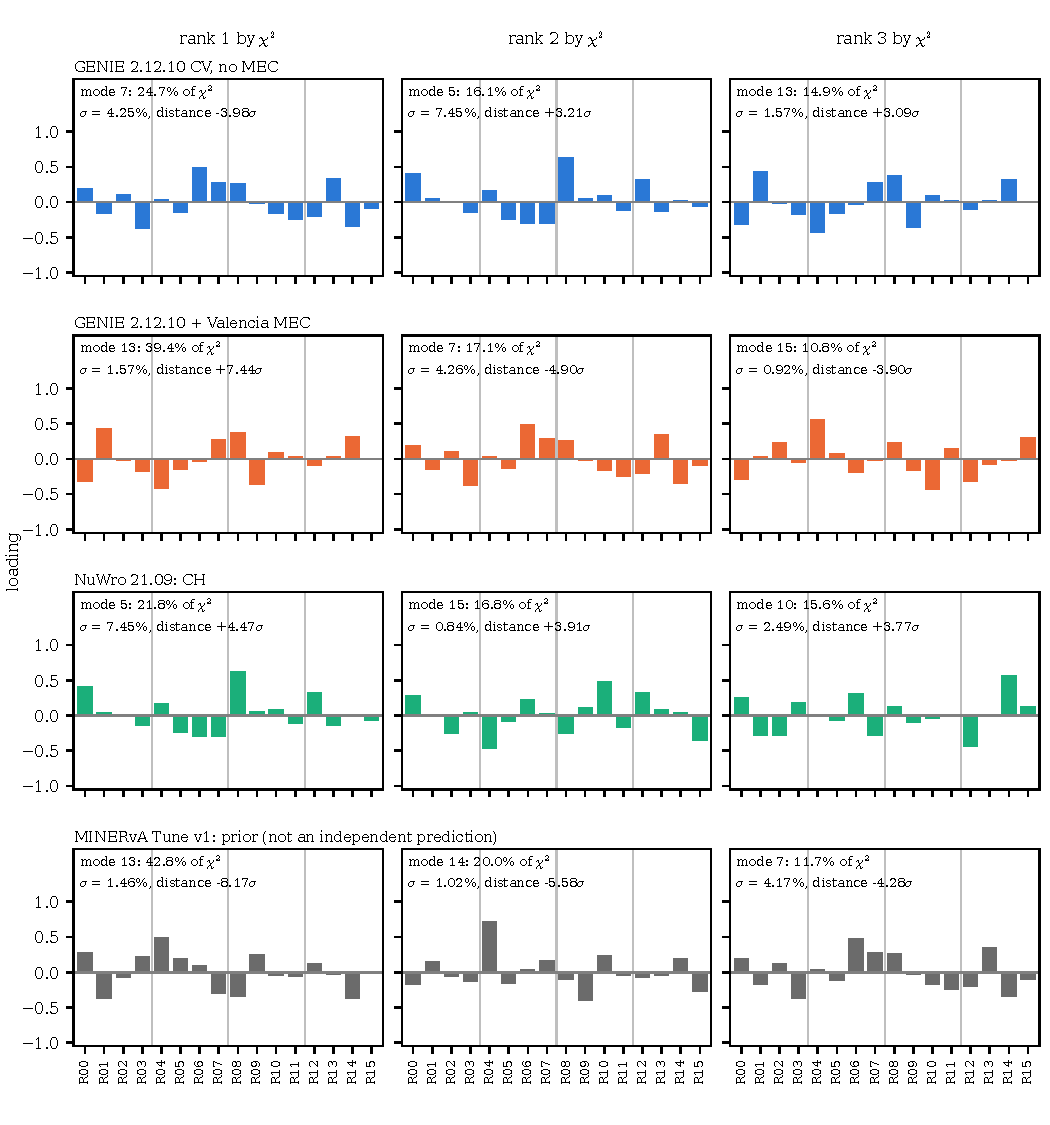
\includegraphics[width=\linewidth]{figures/fd_g_fig_modes.pdf}
\caption[Leading $\chi^2$ modes of the generator comparison]{The leading modes locate where among the sixteen cells each prediction's $\chi^2$ arises. Three leading $\chi^2$ modes (columns, ranked) for GENIE CV, GENIE + MEC, NuWro (corrected to CH, the secondary comparison) and MINERvA Tune~v1 (rows), using $C_{\mathrm{total}}+C_{\mathrm{resp}}+C_{\mathrm{PL,5D}}+V_g$ relative to $f$. Bars: unit loadings on R00--R15, largest loading positive. Panels: $\chi^2$ share, relative $\sigma$, and distance (residual projection/$\sigma$). The residual $(f-g)/f$ makes positive distance mean data above prediction along the signed mode. GiBUU's 8-cell comparison supplies no modes here. Predictions use analysis definitions.}
\label{fig:fived16-modes}
\end{figure}

\begin{table}[htbp]
\centering\footnotesize
\caption[Eigenmode breakdown of the generator $\chi^2$]{The table counts the modes that carry most of each $\chi^2$ and names the top mode's dominant block. Eigenmode breakdown of the $\chi^2$, with NuWro and GiBUU corrected to CH (the secondary comparison): the fewest modes, in $\chi^2$ order, carrying \fvval{diag-fractions}\,\% of it, and the top mode's share of the $\chi^2$, its relative $\sigma$ and its dominant block.}
\label{tab:fived16-diag}
\begin{tabular}{@{}lcccrrl@{}}
\toprule
prediction & \multicolumn{3}{c}{modes for \fvval{diag-fractions}\,\%} & top mode (\% of $\chi^2$) & $\sigma$ (\%) & block \\
\midrule
\fvval{label-gcv} & \fvval{diag-gcv-reported-modes50} & \fvval{diag-gcv-reported-modes90} & \fvval{diag-gcv-reported-modes99} & \fvval{diag-gcv-reported-top-share} & \fvval{diag-gcv-reported-top-sigma} & \fvval{diag-gcv-reported-top-block} \\
\fvval{label-gmec} & \fvval{diag-gmec-reported-modes50} & \fvval{diag-gmec-reported-modes90} & \fvval{diag-gmec-reported-modes99} & \fvval{diag-gmec-reported-top-share} & \fvval{diag-gmec-reported-top-sigma} & \fvval{diag-gmec-reported-top-block} \\
\fvval{label-nuwro} & \fvval{diag-nuwro-reported-modes50} & \fvval{diag-nuwro-reported-modes90} & \fvval{diag-nuwro-reported-modes99} & \fvval{diag-nuwro-reported-top-share} & \fvval{diag-nuwro-reported-top-sigma} & \fvval{diag-nuwro-reported-top-block} \\
\fvval{label-gibuu} & \fvval{diag-gibuu-reported-modes50} & \fvval{diag-gibuu-reported-modes90} & \fvval{diag-gibuu-reported-modes99} & \fvval{diag-gibuu-reported-top-share} & \fvval{diag-gibuu-reported-top-sigma} & \fvval{diag-gibuu-reported-top-block} \\
\fvval{label-tune} & \fvval{diag-tune-reported-modes50} & \fvval{diag-tune-reported-modes90} & \fvval{diag-tune-reported-modes99} & \fvval{diag-tune-reported-top-share} & \fvval{diag-tune-reported-top-sigma} & \fvval{diag-tune-reported-top-block} \\
\bottomrule
\end{tabular}
\end{table}

Cell R04 ($\pT<\fvval{h2-mid-pt}$, $\pPar\geq\fvval{h2-mid-pz}$, $\Eavail<\fvval{h2-mid-eavail}$, $q_3<\fvval{h2-mid-q3}$) has the smallest relative $\sigma$ of the sixteen, \fvval{r04-sigma-total}\,\%, of which flux is the largest group at \fvval{r04-sigma-flux}\,\%. Under the flux block alone its correlation with the \fvval{r04-ncorr} cells that load with it in the top modes is \fvval{r04-corrflux-min}--\fvval{r04-corrflux-max}; under the reported covariance it is \fvval{r04-corr-min}--\fvval{r04-corr-max}.

\subsubsection{The predictions' target and definitions}
\label{sec:fived16-gen-target}
% GENCMP round (DECISION-20261101-joseph-gencmp-paper-adoption.md items 1-4 and 6; director's rulings of 2026-11-01). Sources: FD-GENCMP-REPORT.md sec. 2.1-2.4 (#648) and its readouts fd/gencmp/readout/{defs,ch,native,overlap}.json and receipts/d_projection.txt, each pinned in make_values_fived16.py; the construction and the definitions, FD-GENCMP-DECLARATION.md sec. 2-3 and 5; C_model's samples, nd-unfolding/pv-ladder/config.json:58-65 (the frozen C12 products of the declaration's control A1). The sensitivities, the bootstrap and the modes above are Stage G's chain rerun on Table IV's predictions (GENCMP amendment E, E-1 rerun1: FD-GENCMP-AMENDMENT-E-REPORT.md sec. 3.1, readouts fd/gencmp-e/rerun1/chain/chdefs/); Table tab:fived16-gen-stageg keeps Stage G as first made, from its committed readouts (pin g0 in make_values_fived16.py). C_model's target (DECISION-20261102-joseph-cmodel-keep-carbon-state-effect.md items 2-4): FD-GENCMP-AMENDMENT-E-ADDENDUM-E2-REPORT.md sec. 3 (fd/gencmp-e2/rerun1/chi2/e2.json), sec. 5 (rerun1/sens/x_e2_sens.out.txt) and sec. 7 (the limits), pinned as e2 and e2sens; the reported covariance keeps C_model on carbon.
The predictions of Table~\ref{tab:fived16-gen} differ from the generators' own products in their definitions, and a secondary comparison also changes the target. First, in that secondary comparison NuWro and GiBUU, generated on carbon, are corrected to CH per fine cell as in \S\ref{sec:joint5d-ch}. Second, all four use the analysis definitions of $W$ and of the muon angle: $W$ is computed with the struck nucleon's mass, or an average nucleon mass where the generator records no single struck nucleon, and the muon angle is measured from the beam axis, each event's neutrino direction being drawn from the analysis simulation's distribution in its $E_\nu$ bin. The prediction is the mean over five such draws. With the generators' own definitions restored, every sample reproduces its committed product bit for bit. The change of definitions moves no cell of any of the four by more than \fvval{gdef-dmax} of the cell's reported $\sigma$, and the standard deviation over the five draws is at most \fvval{gdef-seedmax}\,$\sigma$. MINERvA Tune~v1 is already in the analysis definitions and is unchanged.

Table~\ref{tab:fived16-gen-target} gives the CH values and the sensitivities. Corrected to CH, in the analysis definitions, NuWro gives \fvval{g-nuwro-total-chi2} (shape-only \fvval{g-nuwro-shape_only-chi2}) and GiBUU \fvval{g-gibuu-total-chi2} (\fvval{g-gibuu-shape_only-chi2}), against \fvval{g-nuwro-carbon-total-chi2} and \fvval{g-gibuu-carbon-total-chi2} on carbon (Table~\ref{tab:fived16-gen}). The correction lowers NuWro's total $\chi^2$ and raises GiBUU's by \fvval{g-gibuu-chrise}, while GiBUU's shape-only $\chi^2$ falls. In the sixteen-cell comparison GiBUU's total $\chi^2$, on its eight cells, rises, because the CH prediction is paired with $C_{\mathrm{model}}$'s NuWro and GiBUU shape ratios from carbon (below). With the reported $C_{\mathrm{model}}$, that rise also depends on the hydrogen sample: with GENIE CV's hydrogen in place of GiBUU's own, in the generators' own definitions, GiBUU's total is \fvval{g-gibuu-genieh-total-chi2}, below its carbon value of \fvval{g-gibuu-gen-carbon-total-chi2}. GENIE's hydrogen sample is thin, so that spread is largely its own Monte Carlo noise, and the GENIE-hydrogen rows are sensitivities, never the comparison. GiBUU's CH comparison carries the label of \S\ref{sec:joint5d-ch}. The sampling-closure check failed on its hydrogen sample. A bias check of that check's premise, added post hoc, passed at $\le\fvval{g-gibuu-hlab-sigc}\,\sigma_c$. Deep-inelastic events, \fvval{g-gibuu-hlab-dis}\,\% of its hydrogen sample, do not conserve energy.

A native CH generation of NuWro, with only the target changed in the production card, was compared cell by cell with the combination under a rule fixed before the comparison was made: $\sum z^2<\fvval{gnat-rule-sumz2}$ over the sixteen cells and no $|z|>\fvval{gnat-rule-zmax}$, with $z$ from the two samples' Monte Carlo variances. It agrees in the generators' definitions ($\sum z^2=\fvval{gnat-gen-sumz2}$, largest $|z|=\fvval{gnat-gen-zmax}$) and in the analysis definitions (\fvval{gnat-ana-sumz2} and \fvval{gnat-ana-zmax}). Its $\chi^2$ is \fvval{g-nuwro-native-gen-total-chi2} against the combination's \fvval{g-nuwro-gen-ch-total-chi2}; the comparison uses the combination. A diagnostic that was not a test specified before it ran: in one chunk of the generation's probe, NuWro's total cross section per nucleon is \fvval{gnat-probe-pct}\,\% above $(12\sigma_{\mathrm{C}}+\sigma_{\mathrm{H}})/13$ computed from one chunk each of the production carbon sample and the free-proton sample, mostly in deep-inelastic events.

The $C_{\mathrm{model}}$ components of the reported covariance are built from the generators' samples in their own definitions, with NuWro and GiBUU on carbon, not from the predictions of Table~\ref{tab:fived16-gen}. Table~\ref{tab:fived16-gen-cmodel} measures the effect of that target. There, NuWro's and GiBUU's shape ratios in $C_{\mathrm{model}}$ are taken from their CH combinations in the generators' own definitions (the ``CH (generator)'' rows of Table~\ref{tab:fived16-gen-target}), with everything else fixed; the reported covariance keeps them on carbon. Under the reported covariance the total $\chi^2$ changes by $\fvval{e2-with-gcv-total-dch}$ (GENIE CV), $\fvval{e2-with-gmec-total-dch}$ (GENIE + MEC), $\fvval{e2-with-nuwro-total-dch}$ (NuWro) and $\fvval{e2-with-gibuu-total-dch}$ (GiBUU). Over both matrices and both kinds, the largest change is $-\fvval{e2-dmax}$, in GENIE + MEC's shape-only $\chi^2$ without $C_{\mathrm{PL,5D}}$. Only the NuWro and GiBUU components change, but every prediction's $\chi^2$ moves, because the components enter one matrix. With the CH shape ratios, GiBUU's CH total is \fvval{e2-with-gibuu-total-ch}, below its carbon value of \fvval{g-gibuu-carbon-total-chi2} with the reported covariance, so the rise described above comes from pairing the CH prediction with the carbon shape ratios.

For the scale of $C_{\mathrm{model}}$ itself, whose size is not calibrated, the table also gives the $\chi^2$ with $C_{\mathrm{model}}$ removed and doubled. Every $\chi^2$ falls as $C_{\mathrm{model}}$ grows. Removing $C_{\mathrm{model}}$ raises GiBUU's total most, to \fvval{e2-with-gibuu-total-x0} from \fvval{e2-with-gibuu-total-x1}.

With the CH shape ratios, the reported per-cell $\sigma$ falls in \fvval{e2-sig-with-nfall} of the 16 cells and rises in \fvval{e2-sig-with-upcell}, by \fvval{e2-sig-with-up}\,\%. It falls most in \fvval{e2-sig-with-cell}, where $\sigma/f$ goes from \fvval{e2-sig-with-carbon} to \fvval{e2-sig-with-ch} ($-\fvval{e2-sig-with-fall}$\,\%; $-\fvval{e2-sig-nopl-fall}$\,\% without $C_{\mathrm{PL,5D}}$). $C_{\mathrm{model}}$'s own $\sigma/f$ changes most in \fvval{e2-cm-cell}, from \fvval{e2-cm-carbon} to \fvval{e2-cm-ch}, and most in relative terms in \fvval{e2-cm-relcell}, where it is small: from \fvval{e2-cm-relcarbon} to \fvval{e2-cm-relch} ($+\fvval{e2-cm-rel}$\,\%).

This measures $C_{\mathrm{model}}$'s dependence on the target only: its definitions stay the generators' own, its coverage is still not validated, and GiBUU's CH shape ratio carries the hydrogen label of \S\ref{sec:joint5d-ch}. The changes are those of these data; their statistical uncertainty, from the data entering the unfolds that build $C_{\mathrm{model}}$, is not measured. Table~\ref{tab:fived16-gen-stageg}, in App.~\ref{app:devhistory}, gives the comparison as first made, in the generators' own definitions with NuWro and GiBUU on carbon.
% absence-ok: scoping statement about what E2 measures (FD-GENCMP-AMENDMENT-E-ADDENDUM-E2-REPORT.md sec. 4: no addendum declared input resampling, so the data's statistical uncertainty on the vertex unfolds is outside E2), not a claim that a result does not exist

\begin{table}[htbp]
\centering\footnotesize
\caption[CH-corrected generator comparison and its sensitivities]{The CH correction is a secondary comparison, with its sensitivities beside it. The CH-corrected values, a secondary comparison (\S\ref{sec:joint5d-ch}), and the sensitivities of the CH correction. Rows marked (generator) are in the generators' own definitions; the others in the analysis definitions. GENIE CV's hydrogen is a sensitivity only. The native NuWro rows are a check of the combination, which the comparison uses.}
\label{tab:fived16-gen-target}
\begin{tabular}{@{}lcccc@{}}
\toprule
 & \multicolumn{2}{c}{reported covariance} & \multicolumn{2}{c}{without $C_{\mathrm{PL,5D}}$} \\ \cmidrule(lr){2-3}\cmidrule(l){4-5}
prediction & $\chi^2$ & shape-only $\chi^2$ & $\chi^2$ & shape-only $\chi^2$ \\
\midrule
\multicolumn{5}{@{}l}{NuWro~21.09, 16 cells} \\
carbon, Table~\ref{tab:fived16-gen} & \fvval{g-nuwro-carbon-total-chi2} & \fvval{g-nuwro-carbon-shape_only-chi2} & \fvval{g-nuwro-carbon-total-chi2-nopl} & \fvval{g-nuwro-carbon-shape_only-chi2-nopl} \\
CH & \fvval{g-nuwro-total-chi2} & \fvval{g-nuwro-shape_only-chi2} & \fvval{g-nuwro-total-chi2-nopl} & \fvval{g-nuwro-shape_only-chi2-nopl} \\
carbon (generator) & \fvval{g-nuwro-gen-carbon-total-chi2} & \fvval{g-nuwro-gen-carbon-shape_only-chi2} & \fvval{g-nuwro-gen-carbon-total-chi2-nopl} & \fvval{g-nuwro-gen-carbon-shape_only-chi2-nopl} \\
CH (generator) & \fvval{g-nuwro-gen-ch-total-chi2} & \fvval{g-nuwro-gen-ch-shape_only-chi2} & \fvval{g-nuwro-gen-ch-total-chi2-nopl} & \fvval{g-nuwro-gen-ch-shape_only-chi2-nopl} \\
CH, GENIE CV's hydrogen (generator) & \fvval{g-nuwro-genieh-total-chi2} & \fvval{g-nuwro-genieh-shape_only-chi2} & \fvval{g-nuwro-genieh-total-chi2-nopl} & \fvval{g-nuwro-genieh-shape_only-chi2-nopl} \\
native CH (generator) & \fvval{g-nuwro-native-gen-total-chi2} & \fvval{g-nuwro-native-gen-shape_only-chi2} & \fvval{g-nuwro-native-gen-total-chi2-nopl} & \fvval{g-nuwro-native-gen-shape_only-chi2-nopl} \\
native CH & \fvval{g-nuwro-native-ana-total-chi2} & \fvval{g-nuwro-native-ana-shape_only-chi2} & \fvval{g-nuwro-native-ana-total-chi2-nopl} & \fvval{g-nuwro-native-ana-shape_only-chi2-nopl} \\
\midrule
\multicolumn{5}{@{}l}{GiBUU~2019, 8 cells with $\pPar<\fvval{h2-mid-pz}$~GeV/$c$} \\
carbon, Table~\ref{tab:fived16-gen} & \fvval{g-gibuu-carbon-total-chi2} & \fvval{g-gibuu-carbon-shape_only-chi2} & \fvval{g-gibuu-carbon-total-chi2-nopl} & \fvval{g-gibuu-carbon-shape_only-chi2-nopl} \\
CH & \fvval{g-gibuu-total-chi2} & \fvval{g-gibuu-shape_only-chi2} & \fvval{g-gibuu-total-chi2-nopl} & \fvval{g-gibuu-shape_only-chi2-nopl} \\
carbon (generator) & \fvval{g-gibuu-gen-carbon-total-chi2} & \fvval{g-gibuu-gen-carbon-shape_only-chi2} & \fvval{g-gibuu-gen-carbon-total-chi2-nopl} & \fvval{g-gibuu-gen-carbon-shape_only-chi2-nopl} \\
CH (generator) & \fvval{g-gibuu-gen-ch-total-chi2} & \fvval{g-gibuu-gen-ch-shape_only-chi2} & \fvval{g-gibuu-gen-ch-total-chi2-nopl} & \fvval{g-gibuu-gen-ch-shape_only-chi2-nopl} \\
CH, GENIE CV's hydrogen (generator) & \fvval{g-gibuu-genieh-total-chi2} & \fvval{g-gibuu-genieh-shape_only-chi2} & \fvval{g-gibuu-genieh-total-chi2-nopl} & \fvval{g-gibuu-genieh-shape_only-chi2-nopl} \\
\bottomrule
\end{tabular}
\end{table}

\begin{table}[htbp]
\centering\footnotesize
\caption[Generator $\chi^2$ against the size of $C_{\mathrm{model}}$]{The table shows how each $\chi^2$ moves when $C_{\mathrm{model}}$ is removed, doubled or rebuilt from CH ratios. $\chi^2$ for four predictions (Table~\ref{tab:fived16-gen}) with $C_{\mathrm{model}}$ removed ($\times0$), reported ($\times1$), doubled ($\times2$), or NuWro/GiBUU shape ratios changed from carbon to CH, all else fixed. $\Delta_{\mathrm{CH}}$: CH minus reported, from unrounded values. Every $\chi^2$ includes $V_g$; GiBUU uses 8 cells. The CH column is this note's sensitivity, omitted by the methods paper because it uses the free-proton samples of \S\ref{sec:joint5d-ch}. Reported ratios remain carbon.}
\label{tab:fived16-gen-cmodel}
\begin{tabular}{@{}llccccc@{}}
\toprule
prediction & $\chi^2$ & $\times0$ & $\times1$ (reported) & $\times2$ & CH & $\Delta_{\mathrm{CH}}$ \\
\midrule
\multicolumn{7}{@{}l}{reported covariance} \\
\fvval{label-gcv} & total & \fvval{e2-with-gcv-total-x0} & \fvval{e2-with-gcv-total-x1} & \fvval{e2-with-gcv-total-x2} & \fvval{e2-with-gcv-total-ch} & $\fvval{e2-with-gcv-total-dch}$ \\
 & shape-only & \fvval{e2-with-gcv-shape_only-x0} & \fvval{e2-with-gcv-shape_only-x1} & \fvval{e2-with-gcv-shape_only-x2} & \fvval{e2-with-gcv-shape_only-ch} & $\fvval{e2-with-gcv-shape_only-dch}$ \\
\fvval{label-gmec} & total & \fvval{e2-with-gmec-total-x0} & \fvval{e2-with-gmec-total-x1} & \fvval{e2-with-gmec-total-x2} & \fvval{e2-with-gmec-total-ch} & $\fvval{e2-with-gmec-total-dch}$ \\
 & shape-only & \fvval{e2-with-gmec-shape_only-x0} & \fvval{e2-with-gmec-shape_only-x1} & \fvval{e2-with-gmec-shape_only-x2} & \fvval{e2-with-gmec-shape_only-ch} & $\fvval{e2-with-gmec-shape_only-dch}$ \\
\fvval{label-nuwro} & total & \fvval{e2-with-nuwro-total-x0} & \fvval{e2-with-nuwro-total-x1} & \fvval{e2-with-nuwro-total-x2} & \fvval{e2-with-nuwro-total-ch} & $\fvval{e2-with-nuwro-total-dch}$ \\
 & shape-only & \fvval{e2-with-nuwro-shape_only-x0} & \fvval{e2-with-nuwro-shape_only-x1} & \fvval{e2-with-nuwro-shape_only-x2} & \fvval{e2-with-nuwro-shape_only-ch} & $\fvval{e2-with-nuwro-shape_only-dch}$ \\
\fvval{label-gibuu} & total & \fvval{e2-with-gibuu-total-x0} & \fvval{e2-with-gibuu-total-x1} & \fvval{e2-with-gibuu-total-x2} & \fvval{e2-with-gibuu-total-ch} & $\fvval{e2-with-gibuu-total-dch}$ \\
 & shape-only & \fvval{e2-with-gibuu-shape_only-x0} & \fvval{e2-with-gibuu-shape_only-x1} & \fvval{e2-with-gibuu-shape_only-x2} & \fvval{e2-with-gibuu-shape_only-ch} & $\fvval{e2-with-gibuu-shape_only-dch}$ \\
\midrule
\multicolumn{7}{@{}l}{without $C_{\mathrm{PL,5D}}$} \\
\fvval{label-gcv} & total & \fvval{e2-nopl-gcv-total-x0} & \fvval{e2-nopl-gcv-total-x1} & \fvval{e2-nopl-gcv-total-x2} & \fvval{e2-nopl-gcv-total-ch} & $\fvval{e2-nopl-gcv-total-dch}$ \\
 & shape-only & \fvval{e2-nopl-gcv-shape_only-x0} & \fvval{e2-nopl-gcv-shape_only-x1} & \fvval{e2-nopl-gcv-shape_only-x2} & \fvval{e2-nopl-gcv-shape_only-ch} & $\fvval{e2-nopl-gcv-shape_only-dch}$ \\
\fvval{label-gmec} & total & \fvval{e2-nopl-gmec-total-x0} & \fvval{e2-nopl-gmec-total-x1} & \fvval{e2-nopl-gmec-total-x2} & \fvval{e2-nopl-gmec-total-ch} & $\fvval{e2-nopl-gmec-total-dch}$ \\
 & shape-only & \fvval{e2-nopl-gmec-shape_only-x0} & \fvval{e2-nopl-gmec-shape_only-x1} & \fvval{e2-nopl-gmec-shape_only-x2} & \fvval{e2-nopl-gmec-shape_only-ch} & $\fvval{e2-nopl-gmec-shape_only-dch}$ \\
\fvval{label-nuwro} & total & \fvval{e2-nopl-nuwro-total-x0} & \fvval{e2-nopl-nuwro-total-x1} & \fvval{e2-nopl-nuwro-total-x2} & \fvval{e2-nopl-nuwro-total-ch} & $\fvval{e2-nopl-nuwro-total-dch}$ \\
 & shape-only & \fvval{e2-nopl-nuwro-shape_only-x0} & \fvval{e2-nopl-nuwro-shape_only-x1} & \fvval{e2-nopl-nuwro-shape_only-x2} & \fvval{e2-nopl-nuwro-shape_only-ch} & $\fvval{e2-nopl-nuwro-shape_only-dch}$ \\
\fvval{label-gibuu} & total & \fvval{e2-nopl-gibuu-total-x0} & \fvval{e2-nopl-gibuu-total-x1} & \fvval{e2-nopl-gibuu-total-x2} & \fvval{e2-nopl-gibuu-total-ch} & $\fvval{e2-nopl-gibuu-total-dch}$ \\
 & shape-only & \fvval{e2-nopl-gibuu-shape_only-x0} & \fvval{e2-nopl-gibuu-shape_only-x1} & \fvval{e2-nopl-gibuu-shape_only-x2} & \fvval{e2-nopl-gibuu-shape_only-ch} & $\fvval{e2-nopl-gibuu-shape_only-dch}$ \\
\bottomrule
\end{tabular}
\end{table}

% the section's tables (sec:fived16-gen-target) stay before the joint tests begin
\clearpage

